\chapter{Semantica}

\qs{}{Si possono costruire le grammatiche a mano?}

\begin{itemize}
  \item Per l'italiano: L. Lesmo (1985 $\rightarrow$ 2014), Common Lisp.
  \item Per l'inglese: 
    \begin{itemize}
      \item SHRDLU (Winograd 1972). 
      \item CHAT-80 (1979 $\rightarrow$ 1982), sviluppato in Prolog. È un linguaggio naturale per un database sulla geografia.
    \end{itemize}
\end{itemize}

\section{Fondamenti di Semantica Computazionale}


\paragraph{Rappresentare il significato:}

\begin{itemize}
  \item Quale forma per il significato?
    \begin{itemize}
      \item Tavole di un database, logica descrittiva, logica modale, AMR. 
    \end{itemize}
  \item Blackburn e Bos $\rightarrow$ Logica del primordine. 
  \item Il problema nasce per le frasi incomplete. 
  \item Lambda e logica del primordine per parole e sintagmi.
\end{itemize}

\paragraph{Logica del primordine:}

\begin{itemize}
  \item Simboli:
    \begin{itemize}
      \item Costanti. 
      \item Predicati e relazioni. 
      \item Variabili. 
      \item Connettivi logici. 
      \item Quantificatori. 
      \item Altri simboli.
    \end{itemize}
  \item Formule:
    \begin{itemize}
      \item Atomiche. 
      \item Composte. 
      \item Quantificate.
    \end{itemize}
\end{itemize}

\subsection{Algoritmo Fondamentale della Semantica Computazionale}

\begin{enumerate}
  \item Parsificare la frase per ottenere l'albero sintattico. 
  \item Cercare la semantica di ogni persona nel lessico. 
  \item Costruire la semantica per ogni sintagma:
    \begin{itemize}
      \item Bottom-up. 
      \item Syntax-driven: traduzione rule-to-rule.
    \end{itemize}
\end{enumerate}

\dfn{Principio di Composizionalità di Frege}{
  Il significato del tutto è determinato dal significato delle parti e dalla
maniera in cui sono combinate.
}

\begin{figure}[!h]
    \centering
    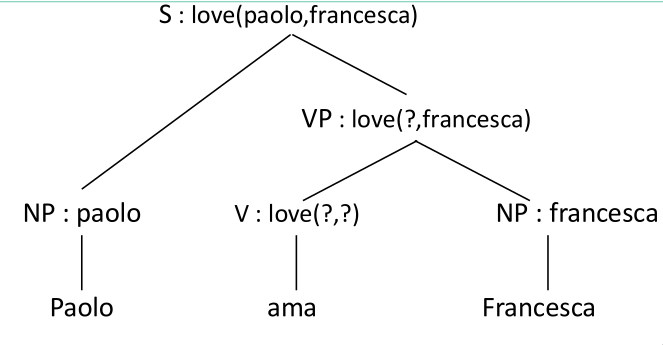
\includegraphics[scale=0.5]{03/Love.png}
    \caption{Applicazione dell'algoritmo.}
\end{figure}

\paragraph{Il significato della frase è costruito:}
\begin{itemize}
  \item Dal significato delle parole $\rightarrow$ Lessico. 
  \item Risalendo le costruzioni semantiche $\rightarrow$ Regole semantiche.
\end{itemize}

\paragraph{Sistematicità:}

\begin{itemize}
  \item Come costruiamo il significato del VP? 
  \item Come specificare in che maniera combinare i pezzi? 
  \item Come rappresentare pezzi di formule?
\end{itemize}

\section{Lambda Astrazione}

\paragraph{Si utilizza il lambda $\lambda$:}

\begin{itemize}
  \item Il nuovo operatore $\lambda$ si usa per legare (bind) le variabili libere. 
  \item Questo simbolo meta-logico segna l'informazione mancante, ossia l'informazione generica.
\end{itemize}

\subsection{Beta riduzione}

$$\lambda (x.love(x, mary)) (john)$$

\begin{itemize}
  \item Si elimina il $\lambda$:
    \begin{itemize}
      \item $(love(x, mary)) (john)$ 
    \end{itemize}
  \item Si rimuove l'argomento:
    \begin{itemize}
      \item $love(x, mary)$
    \end{itemize}
  \item Si rimpiazzano le occorrenze della variabile legata dal $\lambda$ con l'argomento in tutta la formula: 
    \begin{itemize}
      \item $love(john, mary)$
    \end{itemize}
\end{itemize}

\begin{figure}[!h]
    \centering
    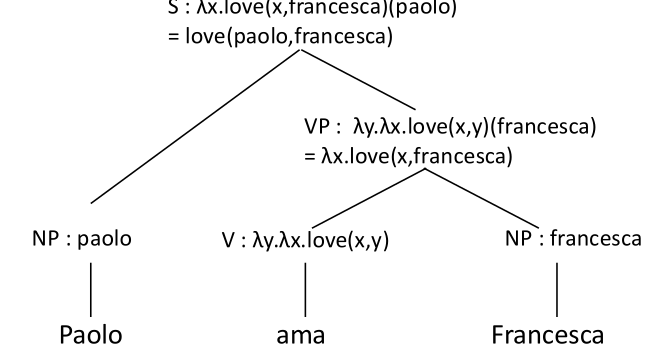
\includegraphics[scale=0.37]{03/Love2.png}
    \caption{Beta riduzione.}
\end{figure}

\subsection{Semantica di Montague}

Montague propose un collegamento tra i linguaggi naturali e la logica: rifiutò dell'assunzione che ci sia una differenza importante tra linguaggi formali e linguaggi naturali. Inoltre viene mostrata l'influenza del tempo a livello del significato (logica temporale):

\begin{itemize}
  \item U: utterance. 
  \item R: reverence. 
  \item E: event.
\end{itemize}

\nt{Queste tre parti si combinano insieme per modificare il significato.}

\begin{figure}[!h]
    \centering
    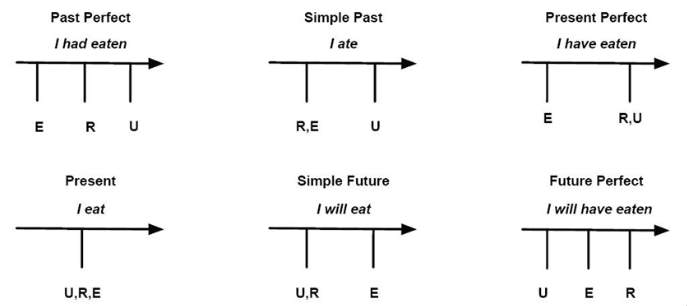
\includegraphics[scale=0.4]{03/tempo.png}
    \caption{Rappresentazione del tempo.}
\end{figure}
\pagebreak
\subsection{Articoli e Nomi Propri}
\begin{figure}[!h]
    \centering
    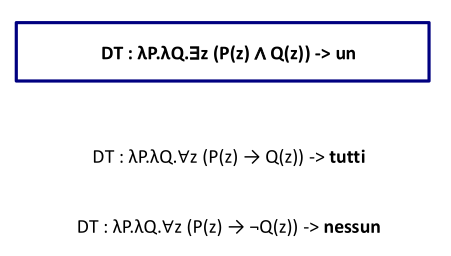
\includegraphics[scale=0.4]{04/quant.png}
    \caption{Rappresentazione degli articoli nel lambda calcolo.}
\end{figure}

\begin{figure}[!h]
    \centering
    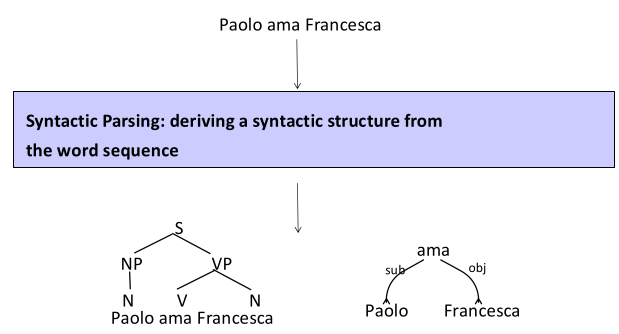
\includegraphics[scale=0.4]{04/paf.png}
    \caption{Esempio di frase con l'articolo "un".}
\end{figure}

\begin{figure}[!h]
    \centering
    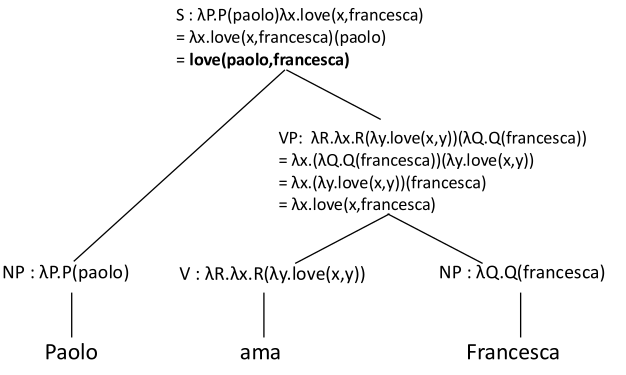
\includegraphics[scale=0.4]{04/paf2.png}
    \caption{Il nuovo modo di trattare i nomi propri.}
\end{figure}

\nt{Attenzione alle ambiguità: \textit{Every man loves a woman}.}

\textbf{Lettura 1:}
\[
\forall x (\text{man}(x) \to \exists y (\text{woman}(y) \wedge \text{love}(x, y)))
\]

\textbf{Lettura 2:}
\[
\exists y (\text{woman}(y) \forall x (\text{man}(x) \to \text{love}(x, y)))
\]

\[
\boxed{\lambda Q \lambda P (\forall x (Q(x) \to P(x))) \to \textbf{Every}}
\]

\subsection{NLTK}

Esiste una libreria in python\footnote{Che schifo python.} per la linguistica computazionale. \fancyglitter{NLTK} (Natural Language ToolKit) è anche un libro pensato per dei linguisti che vogliono imparare a programmare (in python): nei primi capitoli vengono presentate le basi (variabili, cicli, etc.), verso la fine parla di semantica computazionale. Le principali caratteristiche della libreria includono:

\begin{itemize}
  \item Logica del primordine e lambda calcolo. 
  \item Theorem proving, costruzione di modelli e model checking. 
  \item Semantiche varie. 
  \item Logica lineare. 
  \item Altre robe.
\end{itemize}

\begin{lstlisting}[language=Python, caption=Esempio di semantica inglese utilizzando NLTK.]
from nltk import load_parser
parser = load_parser('./simple-sem.fcfg', trace=0)
sentence = 'Angus gives a bone to every dog'
tokens = sentence.split()
for tree in parser.parse(tokens):
  print(tree.label()['SEM'])

all z2.(dog(z2) -> exists z1.(bone(z1) & give(angus,z1,z2)))
\end{lstlisting}


